\documentclass[12pt, a4paper]{article}
\usepackage[utf8]{inputenc}
\usepackage[T1]{fontenc}
\usepackage{amsmath, amssymb}
\usepackage{tikz}
\usetikzlibrary{shapes.gates.logic.US, positioning, calc}
\usepackage[margin=1in]{geometry}
\usepackage[many]{tcolorbox}
\usepackage{enumitem}
\usepackage{microtype}
\usepackage{hyperref} % Added for clickable links

\definecolor{primary}{HTML}{1A365D}   % Deep elegant blue
\definecolor{secondary}{HTML}{C53030} % Professional crimson red
\definecolor{tertiary}{HTML}{2F855A}  % Elegant emerald green for hardware
\definecolor{quaternary}{HTML}{2B6CB0} % Bright blue for circuit box
\definecolor{codecolor}{HTML}{2D3748} % Dark slate gray for code box
\definecolor{accent}{HTML}{2B6CB0}    % Lighter blue for logic states
\definecolor{bglight}{HTML}{F7FAFC}   % Soft off-white for the background

% Configure hyperref to make links look clean
\hypersetup{
    colorlinks=true,
        linkcolor=accent,
	    urlcolor=accent,
	        pdftitle={Digital Logic Hardware Implementation}
		}


		\newtcolorbox{questionbox}{
		    enhanced,
		        colback=bglight,
			    colframe=primary,
			        title=\textbf{Problem \hfill (GATE IN 2022)},
				    coltitle=white,
				        boxrule=1.2pt,
					    arc=6pt,
					        drop shadow=black!10!white,
						    fonttitle=\large,
						        attach boxed title to top left={xshift=5mm, yshift=-3mm},
							    boxed title style={colback=primary, arc=4pt, boxrule=0pt},
							        top=15pt,
								    bottom=10pt,
								        left=15pt,
									    right=15pt
									    }

									    \newtcolorbox{truthtablebox}{
									        enhanced,
										    colback=bglight,
										        colframe=primary,
											    title=\textbf{Truth Table},
											        coltitle=white,
												    boxrule=1.2pt,
												        arc=6pt,
													    drop shadow=black!10!white,
													        fonttitle=\large,
														    attach boxed title to top left={xshift=5mm, yshift=-3mm},
														        boxed title style={colback=primary, arc=4pt, boxrule=0pt},
															    top=15pt,
															        bottom=10pt,
																    left=15pt,
																        right=15pt
																	}

																	\newtcolorbox{solutionbox}{
																	    enhanced,
																	        colback=white,
																		    colframe=secondary,
																		        title=\textbf{Systematic Solution},
																			    coltitle=white,
																			        boxrule=1.2pt,
																				    arc=6pt,
																				        drop shadow=black!10!white,
																					    fonttitle=\large,
																					        attach boxed title to top left={xshift=5mm, yshift=-3mm},
																						    boxed title style={colback=secondary, arc=4pt, boxrule=0pt},
																						        top=15pt,
																							    bottom=10pt,
																							        left=15pt,
																								    right=15pt
																								    }

																								    \newtcolorbox{hardwarebox}{
																								        enhanced,
																									    colback=white,
																									        colframe=tertiary,
																										    title=\textbf{Hardware Implementation},
																										        coltitle=white,
																											    boxrule=1.2pt,
																											        arc=6pt,
																												    drop shadow=black!10!white,
																												        fonttitle=\large,
																													    attach boxed title to top left={xshift=5mm, yshift=-3mm},
																													        boxed title style={colback=tertiary, arc=4pt, boxrule=0pt},
																														    top=15pt,
																														        bottom=10pt,
																															    left=15pt,
																															        right=15pt
																																}

																																\newtcolorbox{circuitbox}{
																																    enhanced,
																																        colback=bglight,
																																	    colframe=quaternary,
																																	        title=\textbf{Circuit Diagram},
																																		    coltitle=white,
																																		        boxrule=1.2pt,
																																			    arc=6pt,
																																			        drop shadow=black!10!white,
																																				    fonttitle=\large,
																																				        attach boxed title to top left={xshift=5mm, yshift=-3mm},
																																					    boxed title style={colback=quaternary, arc=4pt, boxrule=0pt},
																																					        top=15pt,
																																						    bottom=10pt,
																																						        left=15pt,
																																							    right=15pt
																																							    }

																																							    \newtcolorbox{codebox}{
																																							        enhanced,
																																								    colback=white,
																																								        colframe=codecolor,
																																									    title=\textbf{Code Implementation},
																																									        coltitle=white,
																																										    boxrule=1.2pt,
																																										        arc=6pt,
																																											    drop shadow=black!10!white,
																																											        fonttitle=\large,
																																												    attach boxed title to top left={xshift=5mm, yshift=-3mm},
																																												        boxed title style={colback=codecolor, arc=4pt, boxrule=0pt},
																																													    top=15pt,
																																													        bottom=15pt,
																																														    left=15pt,
																																														        right=15pt
																																															}

																																															\pagestyle{empty}
																																															\begin{document}

																																														
																																															\begin{questionbox}
																																															    \textbf{Q43.} The logic block shown in Fig. 3.25 has an output $F$ given by \underline{\hspace{3cm}}.
																																															        
																																																    \vspace{0.5cm}
																																																        \begin{center}
																																																	        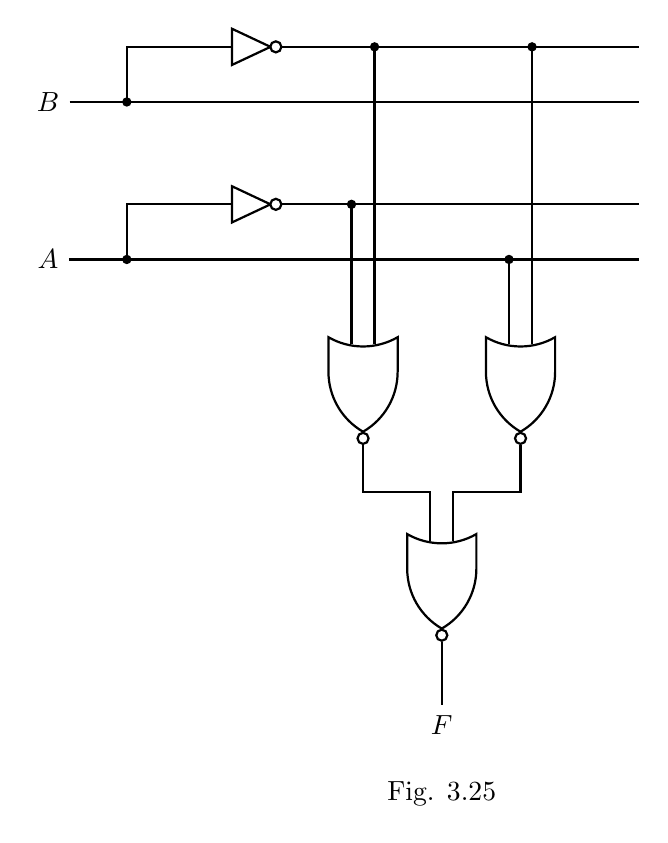
\begin{tikzpicture}[
																																																		            logic gate inputs=nn,
																																																			                thick,
																																																					            gate/.style={draw, minimum size=2.5em},
																																																						                dot/.style={circle, fill, inner sep=1.2pt}
																																																								        ]
																																																									        
																																																										        % Inputs A & B
																																																											        \node (B) at (0, 2.5) {$B$};
																																																												        \node (A) at (0, 0.5) {$A$};

																																																													        % Horizontal source lines
																																																														        \draw (B) -- (7.5, 2.5);
																																																															        \draw (A) -- (7.5, 0.5);

																																																																        % NOT gates
																																																																	        \node[not gate US, draw, thick] (notB) at (2.5, 3.2) {};
																																																																		        \node[not gate US, draw, thick] (notA) at (2.5, 1.2) {};

																																																																			        % Connections going into NOT gates
																																																																				        \draw (1, 2.5) node[dot]{} |- (notB.input);
																																																																					        \draw (1, 0.5) node[dot]{} |- (notA.input);

																																																																						        % Output lines from NOT gates
																																																																							        \draw (notB.output) -- (7.5, 3.2);
																																																																								        \draw (notA.output) -- (7.5, 1.2);

																																																																									        % --- First Stage NOR gates ---
																																																																										        \node[nor gate US, draw, thick, rotate=-90, minimum size=2.5em] (nor1) at (4, -1) {};
																																																																											        \node[nor gate US, draw, thick, rotate=-90, minimum size=2.5em] (nor2) at (6, -1) {};

																																																																												        % Wiring Left NOR (nor1)
																																																																													        \draw (nor1.input 2) -- (nor1.input 2 |- 0, 1.2) node[dot]{}; % connects to A_bar
																																																																														        \draw (nor1.input 1) -- (nor1.input 1 |- 0, 3.2) node[dot]{}; % connects to B_bar

																																																																															        % Wiring Right NOR (nor2)
																																																																																        \draw (nor2.input 2) -- (nor2.input 2 |- 0, 0.5) node[dot]{}; % connects to A
																																																																																	        \draw (nor2.input 1) -- (nor2.input 1 |- 0, 3.2) node[dot]{}; % connects to B_bar

																																																																																		        % --- Final NOR gate ---
																																																																																			        \node[nor gate US, draw, thick, rotate=-90, minimum size=2.5em] (nor3) at (5, -3.5) {};

																																																																																				        % Wiring Final NOR
																																																																																					        \draw (nor1.output) -- ++(0, -0.6) -| (nor3.input 2);
																																																																																						        \draw (nor2.output) -- ++(0, -0.6) -| (nor3.input 1);

																																																																																							        % Final Output F
																																																																																								        \draw (nor3.output) -- ++(0, -0.8) node[below] {$F$};

																																																																																									        \node[below] at (5, -6) {Fig. 3.25};
																																																																																										        \end{tikzpicture}
																																																																																											    \end{center}

																																																																																											        \vspace{0.1cm}
																																																																																												    \begin{enumerate}[label=\textbf{\alph*)}, itemsep=0.4em]
																																																																																												            \item $A + B$
																																																																																													            \item $A\bar{B}$
																																																																																														            \item $A + \bar{B}$
																																																																																															            \item $\bar{B}$
																																																																																																        \end{enumerate}
																																																																																																	\end{questionbox}

																																																																																																
																																																																																																	\vspace{0.5cm}
																																																																																																	\begin{truthtablebox}
																																																																																																	    \begin{center}
																																																																																																	            \renewcommand{\arraystretch}{1.4}
																																																																																																		            \setlength{\tabcolsep}{15pt}
																																																																																																			            \begin{tabular}{|c|c||c|c||c|}
																																																																																																				                \hline
																																																																																																						            \textbf{A} & \textbf{B} & $\mathbf{Y_1 = AB}$ & $\mathbf{Y_2 = \bar{A}B}$ & $\mathbf{F = \overline{Y_1 + Y_2}}$ \\
																																																																																																							                \hline
																																																																																																									            0 & 0 & 0 & 0 & \textbf{1} \\
																																																																																																										                0 & 1 & 0 & 1 & \textbf{0} \\
																																																																																																												            1 & 0 & 0 & 0 & \textbf{1} \\
																																																																																																													                1 & 1 & 1 & 0 & \textbf{0} \\
																																																																																																															            \hline
																																																																																																																            \end{tabular}
																																																																																																																	        \end{center}
																																																																																																																		\end{truthtablebox}

																																																																																																																		\newpage % <--- This forces the Solution Box to Page 2
																																																																																																																	
																																																																																																																		\begin{solutionbox}
																																																																																																																		    \textbf{Step 1: Signal Identification on the Main Buses} \\
																																																																																																																		        The circuit generates inverted signals using the two NOT gates. Let's establish the signals on the four horizontal lines from top to bottom:
																																																																																																																			    \begin{itemize}[itemsep=0.2em]
																																																																																																																			            \item \textbf{Line 1 (Top):} Output of the top NOT gate $\implies \mathbf{\bar{B}}$
																																																																																																																				            \item \textbf{Line 2:} Direct input line for $\implies \mathbf{B}$
																																																																																																																					            \item \textbf{Line 3:} Output of the bottom NOT gate $\implies \mathbf{\bar{A}}$
																																																																																																																						            \item \textbf{Line 4 (Bottom):} Direct input line for $\implies \mathbf{A}$
																																																																																																																							        \end{itemize}

																																																																																																																								    \vspace{0.3cm}
																																																																																																																								        \textbf{Step 2: Analysis of the First-Stage NOR Gates} \\
																																																																																																																									    By tracing the vertical lines from the horizontal buses to the inputs of the two parallel NOR gates, we can derive their Boolean expressions:
																																																																																																																									        
																																																																																																																										    \begin{itemize}
																																																																																																																										            \item \textbf{Left NOR Gate ($Y_1$):} \\
																																																																																																																											            The inputs are connected to \textbf{Line 3} ($\bar{A}$) and \textbf{Line 1} ($\bar{B}$). \\
																																																																																																																												            Applying the NOR operation and De Morgan's Law:
																																																																																																																													            $$ Y_1 = \overline{\bar{A} + \bar{B}} = \overline{\overline{A}} \cdot \overline{\overline{B}} = \mathbf{A \cdot B} $$
																																																																																																																														            
																																																																																																																															            \item \textbf{Right NOR Gate ($Y_2$):} \\
																																																																																																																																            The inputs are connected to \textbf{Line 4} ($A$) and \textbf{Line 1} ($\bar{B}$). \\
																																																																																																																																	            Applying the NOR operation:
																																																																																																																																		            $$ Y_2 = \overline{A + \bar{B}} = \overline{A} \cdot \overline{\overline{B}} = \mathbf{\bar{A} \cdot B} $$
																																																																																																																																			        \end{itemize}

																																																																																																																																				    \textbf{Step 3: Evaluating the Final Output ($F$)} \\
																																																																																																																																				        The final NOR gate evaluates the outputs $Y_1$ and $Y_2$:
																																																																																																																																					    \begin{align*}
																																																																																																																																					            F &= \overline{Y_1 + Y_2} \\
																																																																																																																																						              &= \overline{(AB) + (\bar{A}B)} \\
																																																																																																																																							          \end{align*}
																																																																																																																																								      Factor out the common term $B$:
																																																																																																																																								          \begin{align*}
																																																																																																																																									          F &= \overline{B(A + \bar{A})} \\
																																																																																																																																										      \end{align*}
																																																																																																																																										          According to Boolean algebra rules, the OR of a variable with its complement is always $1$ ($A + \bar{A} = 1$):
																																																																																																																																											      \begin{align*}
																																																																																																																																											              F &= \overline{B \cdot 1} \\
																																																																																																																																												              \mathbf{F} &= \mathbf{\bar{B}}
																																																																																																																																													          \end{align*}

																																																																																																																																														      \begin{center}
																																																																																																																																														              \fcolorbox{secondary}{bglight}{\parbox{0.5\textwidth}{
																																																																																																																																															                  \centering \vspace{0.15cm}
																																																																																																																																																	              \textbf{\large Correct Option: (d) $\bar{B}$}
																																																																																																																																																		                  \vspace{0.15cm}
																																																																																																																																																				          }}
																																																																																																																																																					      \end{center}
																																																																																																																																																					      \end{solutionbox}

																																																																																																																																																					      \newpage

																																																																																																																																																					      \begin{hardwarebox}
																																																																																																																																																					          \textbf{1. Components Required}
																																																																																																																																																						      \begin{itemize}[itemsep=0.1em]
																																																																																																																																																						              \item 1x Arduino (Uno/Nano)
																																																																																																																																																							              \item 1x Breadboard
																																																																																																																																																								              \item 1x 7447 Decoder (BCD to 7-Segment)
																																																																																																																																																									              \item 1x Common Anode 7-Segment Display
																																																																																																																																																										              \item 7x $220\Omega$ Resistors (Current limiting for the display segments)
																																																																																																																																																											              \item Jumper Wires
																																																																																																																																																												          \end{itemize}

																																																																																																																																																													      \vspace{0.4cm}
																																																																																																																																																													          \textbf{2. Circuit Connections} 
																																																																																																																																																														      
																																																																																																																																																														          \vspace{0.2cm}
																																																																																																																																																															      \textbf{A. Decoder (7447) to Arduino (Inputs):} \\
																																																																																																																																																															          The 7447 decoder has 4 BCD input pins (A, B, C, D). Since our logic circuit's final output $F$ evaluates to only a single bit (0 or 1), we exclusively need to control Input A (the Least Significant Bit).
																																																																																																																																																																      \begin{itemize}[itemsep=0.1em]
																																																																																																																																																																              \item \textbf{7447 Input A (Pin 7):} Connect to \textbf{Arduino Pin 4} (This pin carries our computed Output $F$).
																																																																																																																																																																	              \item \textbf{7447 Inputs B (Pin 1), C (Pin 2), D (Pin 6):} Connect all directly to \textbf{GND}.
																																																																																																																																																																		              \item \textbf{7447 LT / Pin 3 (Lamp Test):} Connect to \textbf{5V} (This pin is active-low, so connecting it to 5V ensures normal operation).
																																																																																																																																																																			              \item \textbf{7447 BI/RBO / Pin 4 (Blanking):} Connect to \textbf{5V}.
																																																																																																																																																																				              \item \textbf{7447 RBI / Pin 5 (Ripple Blanking):} Connect to \textbf{5V}.
																																																																																																																																																																					              \item \textbf{7447 VCC (Pin 16):} Connect to \textbf{5V}.
																																																																																																																																																																						              \item \textbf{7447 GND (Pin 8):} Connect to \textbf{GND}.
																																																																																																																																																																							          \end{itemize}

																																																																																																																																																																								      \vspace{0.4cm}
																																																																																																																																																																								          \textbf{B. Decoder to 7-Segment Display (Outputs):} \\
																																																																																																																																																																									      Each output pin from the 7447 decoder connects to the corresponding segment of the display through a $220\Omega$ resistor to prevent LED burnout.
																																																																																																																																																																									          \begin{itemize}[itemsep=0.1em]
																																																																																																																																																																										          \item \textbf{7447 Pin 13} $\rightarrow$  \textbf{Segment A}
																																																																																																																																																																											          \item \textbf{7447 Pin 12} $\rightarrow$  \textbf{Segment B}
																																																																																																																																																																												          \item \textbf{7447 Pin 11} $\rightarrow$  \textbf{Segment C}
																																																																																																																																																																													          \item \textbf{7447 Pin 10} $\rightarrow$  \textbf{Segment D}
																																																																																																																																																																														          \item \textbf{7447 Pin 9}  $\rightarrow$  \textbf{Segment E}
																																																																																																																																																																															          \item \textbf{7447 Pin 15} $\rightarrow$  \textbf{Segment F}
																																																																																																																																																																																          \item \textbf{7447 Pin 14} $\rightarrow$  \textbf{Segment G}
																																																																																																																																																																																	          \item \textbf{Display Common Pin:} Connect directly to \textbf{5V}.
																																																																																																																																																																																		      \end{itemize}
																																																																																																																																																																																		      \end{hardwarebox}

																																																																																																																																																																																		      \newpage

																																																																																																																																																																																		
																																																																																																																																																																																		      \begin{circuitbox}
																																																																																																																																																																																		          \begin{center}
																																																																																																																																																																																			          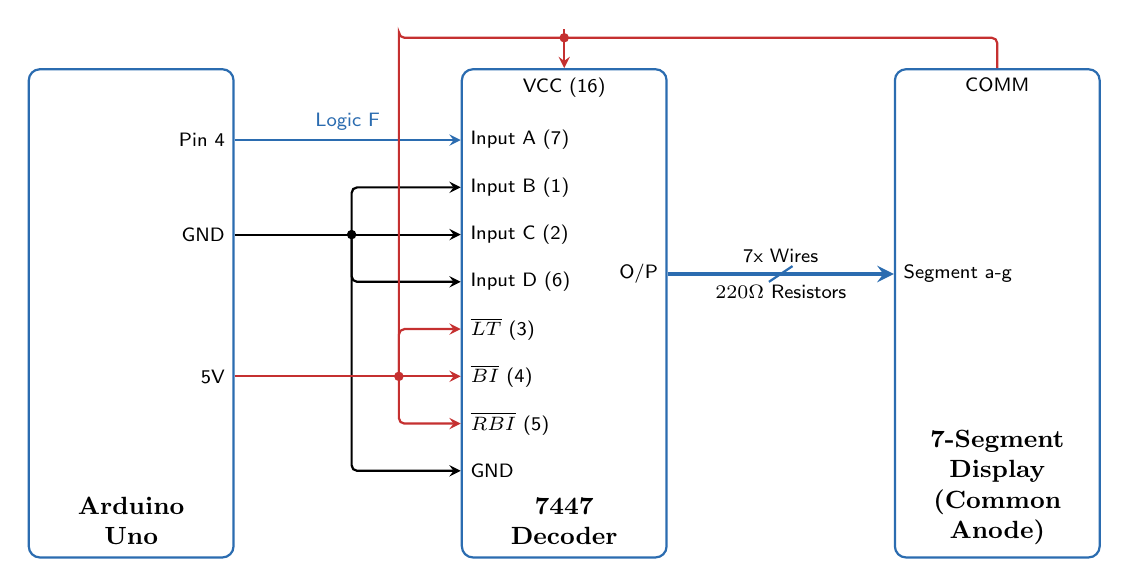
\begin{tikzpicture}[
																																																																																																																																																																																				              >=stealth,
																																																																																																																																																																																					                  box/.style={draw=quaternary, thick, fill=white, rounded corners=4pt, minimum width=2.6cm, minimum height=6.2cm},
																																																																																																																																																																																							              lbl/.style={font=\scriptsize\sffamily},
																																																																																																																																																																																								                  wire/.style={thick, rounded corners=2pt}
																																																																																																																																																																																										          ]
																																																																																																																																																																																											          
																																																																																																																																																																																												          % The three main components (Empty boxes to avoid text overlapping pins)
																																																																																																																																																																																													          \node[box] (arduino) at (0, 0) {};
																																																																																																																																																																																														          \node[box] (decoder) at (5.5, 0) {};
																																																																																																																																																																																															          \node[box] (display) at (11, 0) {};

																																																																																																																																																																																																          % Component Labels placed exactly at the bottom interior of the boxes
																																																																																																																																																																																																	          \node[font=\small\bfseries, align=center, anchor=south] at ([yshift=0.5mm]arduino.south) {Arduino\\Uno};
																																																																																																																																																																																																		          \node[font=\small\bfseries, align=center, anchor=south] at ([yshift=0.5mm]decoder.south) {7447\\Decoder};
																																																																																																																																																																																																			          \node[font=\small\bfseries, align=center, anchor=south] at ([yshift=0.5mm]display.south) {7-Segment\\Display\\(Common\\Anode)};

																																																																																																																																																																																																				          % Arduino Pins Labels
																																																																																																																																																																																																					          \node[lbl, left] at (arduino.east |- 0, 2.2) {Pin 4};
																																																																																																																																																																																																						          \node[lbl, left] at (arduino.east |- 0, 1.0) {GND};
																																																																																																																																																																																																							          \node[lbl, left] at (arduino.east |- 0, -0.8) {5V};

																																																																																																																																																																																																								          % Decoder Pins (Left) Labels (Spread out individually)
																																																																																																																																																																																																									          \node[lbl, right] at (decoder.west |- 0, 2.2) {Input A (7)};
																																																																																																																																																																																																										          \node[lbl, right] at (decoder.west |- 0, 1.6) {Input B (1)};
																																																																																																																																																																																																											          \node[lbl, right] at (decoder.west |- 0, 1.0) {Input C (2)};
																																																																																																																																																																																																												          \node[lbl, right] at (decoder.west |- 0, 0.4) {Input D (6)};
																																																																																																																																																																																																													          \node[lbl, right] at (decoder.west |- 0, -0.2) {$\overline{LT}$ (3)};
																																																																																																																																																																																																														          \node[lbl, right] at (decoder.west |- 0, -0.8) {$\overline{BI}$ (4)};
																																																																																																																																																																																																															          \node[lbl, right] at (decoder.west |- 0, -1.4) {$\overline{RBI}$ (5)};
																																																																																																																																																																																																																          \node[lbl, right] at (decoder.west |- 0, -2.0) {GND};
																																																																																																																																																																																																																	          
																																																																																																																																																																																																																		          % Decoder VCC Pin
																																																																																																																																																																																																																			          \node[lbl, below] at (decoder.north) {VCC (16)};

																																																																																																																																																																																																																				          % Decoder Pins (Right) Labels
																																																																																																																																																																																																																					          \node[lbl, left] at (decoder.east |- 0, 0.5) {O/P};

																																																																																																																																																																																																																						          % Display Pins (Left) Labels
																																																																																																																																																																																																																							          \node[lbl, right] at (display.west |- 0, 0.5) {Segment a-g};

																																																																																																																																																																																																																								          % --- WIRING PATHS ---
																																																																																																																																																																																																																									          
																																																																																																																																																																																																																										          % Data line (Pin 4 to Input A)
																																																																																																																																																																																																																											          \draw[->, wire, draw=accent] (arduino.east |- 0, 2.2) -- (decoder.west |- 0, 2.2) node[midway, above, lbl, text=accent] {Logic F};
																																																																																																																																																																																																																												          
																																																																																																																																																																																																																													          % GND connections (Black) - Branched to individual pins
																																																																																																																																																																																																																														          \draw[->, wire, draw=black] (arduino.east |- 0, 1.0) -- (decoder.west |- 0, 1.0); % Main line to Input C
																																																																																																																																																																																																																															          \draw[->, wire, draw=black] (2.8, 1.0) |- (decoder.west |- 0, 1.6); % Branch to Input B
																																																																																																																																																																																																																																          \draw[->, wire, draw=black] (2.8, 1.0) |- (decoder.west |- 0, 0.4); % Branch to Input D
																																																																																																																																																																																																																																	          \draw[->, wire, draw=black] (2.8, 1.0) |- (decoder.west |- 0, -2.0); % Branch to GND
																																																																																																																																																																																																																																		          \filldraw[black] (2.8, 1.0) circle (1.5pt); % Junction dot for GND
																																																																																																																																																																																																																																			          
																																																																																																																																																																																																																																				          % 5V connections (Red/Secondary) - Branched to individual pins
																																																																																																																																																																																																																																					          \draw[->, wire, draw=secondary] (arduino.east |- 0, -0.8) -- (decoder.west |- 0, -0.8); % Main line to BI
																																																																																																																																																																																																																																						          \draw[->, wire, draw=secondary] (3.4, -0.8) |- (decoder.west |- 0, -0.2); % Branch to LT
																																																																																																																																																																																																																																							          \draw[->, wire, draw=secondary] (3.4, -0.8) |- (decoder.west |- 0, -1.4); % Branch to RBI
																																																																																																																																																																																																																																								          \filldraw[secondary] (3.4, -0.8) circle (1.5pt); % Junction dot for 5V
																																																																																																																																																																																																																																									          % VCC and Display COM to 5V power line
																																																																																																																																																																																																																																										          \draw[wire, draw=secondary] (3.4, -0.8) |- ++(0, 4.3) -| (display.north) node[pos=1, below, lbl] {COMM};
																																																																																																																																																																																																																																											          \draw[<-, wire, draw=secondary] (decoder.north) -- ++(0, 0.5); 
																																																																																																																																																																																																																																												          \filldraw[secondary] (5.5, 3.5) circle (1.5pt); % Junction dot for VCC line

																																																																																																																																																																																																																																													          % Bus line from Decoder to Display
																																																																																																																																																																																																																																														          \draw[->, ultra thick, draw=quaternary] (decoder.east |- 0, 0.5) -- (display.west |- 0, 0.5) node[midway, above, lbl] {7x Wires} node[midway, below, lbl] {$220\Omega$ Resistors};
																																																																																																																																																																																																																																															          \draw[thick, draw=quaternary] (8.1, 0.4) -- (8.4, 0.6); % Slash mark to indicate a bus

																																																																																																																																																																																																																																																          \end{tikzpicture}
																																																																																																																																																																																																																																																	      \end{center}
																																																																																																																																																																																																																																																	          
																																																																																																																																																																																																																																																		      \vspace{0.4cm}
																																																																																																																																																																																																																																																		          \hrule
																																																																																																																																																																																																																																																			      \vspace{0.3cm}
																																																																																																																																																																																																																																																			          
																																																																																																																																																																																																																																																				      \textbf{Overview:} This block diagram illustrates the complete hardware integration. The Arduino Uno computes the Boolean logic and sends the resulting single-bit output ($F$) from Pin 4 to the 7447 decoder's Input A. The decoder translates this binary signal into a 7-segment format, driving the common-anode display via $220\Omega$ current-limiting resistors.
																																																																																																																																																																																																																																																				      \end{circuitbox}

																																																																																																																																																																																																																																																			
																																																																																																																																																																																																																																																				      \vspace{0.5cm}
																																																																																																																																																																																																																																																				      \begin{codebox}
																																																																																																																																																																																																																																																				          \centering
																																																																																																																																																																																																																																																					      \large The full automated Arduino C++ and Assembly code simulating the truth table logic and driving the decoder is available online. \\
																																																																																																																																																																																																																																																					          \vspace{0.4cm}
																																																																																																																																																																																																																																																						      
																																																																																																																																																																																																																																																						          % Simple text link
																																																																																																																																																																																																																																																							      \textbf{\href{https://github.com/Devang0124/Gate-2022-Logic-Hardware/blob/main/gate_logic.ino}{https://github.com/Devang0124/Gate-2022-Logic-Hardware/blob/main/gate\_logic.ino}}
																																																																																																																																																																																																																																																							      \vspace{0.5cm}
																																																																																																																																																																																																																																																								  \textbf{\href{ https://github.com/Devang0124/Gate-2022-Logic-Hardware/blob/main/gate_logic2.asm}{ https://github.com/Devang0124/Gate-2022-Logic-Hardware/blob/main/gate\_logic2.asm}}
																																																																																																																																																																																																																																																							      \end{codebox}

																																																																																																																																																																																																																																																							      \end{document}
